\section{Visualisation and Real-Time Application}

\subsection{Resnet-18 Performance}

\begin{figure}[h]
    \centering
    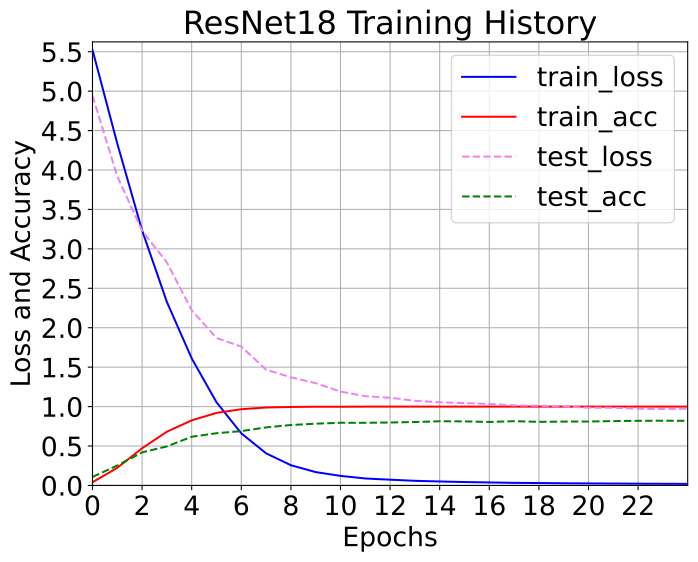
\includegraphics[width=0.5\textwidth]{Resnet18_performance.png}
    \caption{Resnet18 performance}
    \label{fig:resnet18_performance}
\end{figure}

Figure \ref{fig:resnet18_performance} demonstrates that with 25 epochs, the face recognition model Resnet-18 achieves 99.98\% accuracy on the training set and 81.93\% accuracy on the test set. We halted training at this point because any additional epoch would result in an overtraining problem.

\subsection{PGD Attack Real-Time Application}

Using the method described in the preceding section, we developed a program to execute PGD attacks through the camera in real time using the method described in the previous section. Before feeding them into the machine learning model, the application would capture images from the camera and then subject them to PGD perturbations. The output of the model would be monitored and the probability of the prediction would be displayed on the screen. This method allows for the testing and evaluation of machine learning models' resistance to PGD attacks in real time.

% [TODO] Add a screenshot of the interface


